% smp_report.tex — Xinu Pi 5 上の並列実行方式の比較（ワーカーズ型 対 対称SMP型）
%   組版:  lualatex smp_report.tex   （2回）
%   図は pgfplots で描く。数値は本文中にそのまま残るので、原稿が実測値の一次資料になる。
\documentclass[a4paper,11pt]{ltjsarticle}
\usepackage{luatexja}
\usepackage{geometry}
\geometry{margin=25mm}
\usepackage{amsmath}
\usepackage{booktabs}
\usepackage{listings}
\usepackage{xcolor}
\usepackage{pgfplots}
\pgfplotsset{compat=1.18}
\usepackage{caption}
\usepackage{hyperref}
\hypersetup{colorlinks=true,linkcolor=blue!50!black,urlcolor=blue!50!black}

\lstset{
  basicstyle=\ttfamily\scriptsize,
  breaklines=true,
  frame=single,
  framesep=3pt,
  rulecolor=\color{black!30},
  backgroundcolor=\color{black!3},
  columns=fullflexible,
  keepspaces=true,
  showstringspaces=false,
}

% AIPL アクター並列: 粒度 vs 1メッセージあたりの費用[us]（実測・中央値）
\def\aiplW{(1,3.562) (10,8.938) (50,36.719) (200,141.906) (1000,699.500) (5000,3487.062) (20000,13954.625) (100000,69764.094) (200000,139695.688)}
\def\aiplS{(1,5.312) (10,11.688) (50,39.625) (200,144.812) (1000,704.093) (5000,3505.875) (20000,14005.000) (100000,70009.500) (200000,140007.625)}
\def\aiplRatio{(1,1.4914) (10,1.3077) (50,1.0791) (200,1.0205) (1000,1.0066) (5000,1.0054) (20000,1.0036) (100000,1.0035) (200000,1.0022)}

% 実験2: バッチ長 vs 1メッセージあたりの費用[us]（粒度1000・実測）
\def\batW{(2,1072.50) (4,686.00) (8,699.12) (16,740.28) (23,581.65)}
\def\batS{(2,1093.00) (4,690.88) (8,705.69) (16,746.75) (23,590.27)}
% 実験3: 不揃いな仕事（1バッチあたりの makespan [ms]）
\def\unevenW{(1,505.06)}
\def\unevenS{(1,403.06)}

\def\spreadW{(1,89.3) (2,119.0) (4,148.1) (8,175.1) (16,199.5) (32,220.8) (64,238.5) (128,253.4)}
\def\spreadS{(1,89.8) (2,107.0) (4,125.2) (8,143.4) (16,160.8) (32,176.7) (64,190.6) (128,202.5)}
\def\spreadR{(1,0.994) (2,1.112) (4,1.183) (8,1.221) (16,1.241) (32,1.250) (64,1.251) (128,1.251)}
\def\bOneW{(4,144.8) (8,122.6) (16,113.0)}
\def\bOneS{(4,119.7) (8,108.4) (16,105.5)}
\def\bTwoW{(4,144.7) (8,154.4) (16,166.8)}
\def\bTwoS{(4,119.7) (8,125.7) (16,134.6)}
\def\coreUs{(2,2.163) (3,2.428) (4,2.731)}


\title{Xinu Pi 上の並列実行方式の比較\\
\large ワーカーズ型（郵便箱・静的分割）対 対称SMP型（共有 ready キュー）\\
\normalsize ---- N-Queens・通常の並列計算・AIPL アクター並列の実測（Pi 5 / Pi 4 / Pi 3）}
\author{児玉研究室}
\date{2026年9月10日}

\begin{document}
\maketitle

\begin{abstract}
Raspberry Pi 5 / 4 / 3 上のベアメタル Xinu に、並列実行の二方式 ----
核0が各二次コアの郵便箱へ仕事を静的に配る\textbf{ワーカーズ型}と、
各コアが共有 ready キューから自分で取る\textbf{対称SMP型}---- を実装し、
N-Queens・通常の並列計算・\textbf{AIPL のアクター並列}で比較した。

\textbf{ワーカーズ型については測定が完結した。}静的分割の makespan モデルは
実測に $5\%$ 前後で追随し、\textbf{A76 と A72 で比の曲線がほぼ一致する}。
静的分割の弱点は「静的であること」ではなく\textbf{分割の粗さ}であり、
重い仕事が散らばっていれば分割数を増やすだけで理想に近づく
（$301.5 \to 235.3$ ms）。仕事を完全に等量にしても 4 コアで 4 倍は出ず
（2$\to$4 コアで 1 反復が $+27.7\%$）、N-Queens が $2.2\times$ 止まりだった主因はここにある。

\textbf{一方、対称SMP型と AIPL の比較は取れなかった} ---- その経路が正しく動かないためである。
検算計器を入れると誤答・停止・板の死が現れた。時間の行き先を分解した結果、
原因は\textbf{呼び手が自分の持ち分を計算すると先取りで 1 ティックずつ失う}ことにあり
（$399$ 回の先取り $\times\ 10.4$ ms $=4.15$ 秒、\texttt{inline\_us} と一致）、
生成した単位そのものは 1.85 ms で完了していた。
静的分割では自然な「呼び手も 1 単位ぶん働く」設計が、動的スケジューラの上では
20 倍の劣化を招く。\textbf{初稿の「不揃いな仕事では対称SMP型が 1.25 倍速い」は撤回する。}

測定の過程で、例外処理が \texttt{ELR\_EL1}/\texttt{SPSR\_EL1} を保存していないという
カーネルの重大な不具合を Pi 5 と Pi 4 の双方で発見・修正した
（先取りを有効にすると 8 プロセス中 8 個すべてが誤った答えを返す）。
Pi 3 は ARM32 で、同じ状態をスレッド自身のスタックに積んでおり、この穴は無かった。
また\textbf{自分の測定手順にも 3 つの穴}（正誤の未確認・標本が 2 ラウンドで停止・
冷間始動の過渡）を見つけ、いずれも計器を足して塞いだうえで全実験を測り直した。
\end{abstract}

\section{目的と仮説}

我々の研究は、Xinu Pi の上で AIPL を実行することを目的としている。そのための
マルチプロセッサ構成として、\textbf{ワーカーズ型が効率的である}というのが作業仮説である。
本報告はこの仮説を実機で検証する。

主張を「速い」で終わらせず、\textbf{なぜ速いのか}を機構で説明できる形にした。すなわち
1 メッセージあたりの費用を
\[
  \text{us/msg} \;=\; \underbrace{a}_{\text{配布コスト}} \;+\; \underbrace{b \times (\text{粒度})}_{\text{本体の実行}}
\]
と分解し、両方式で $a$ を比較する ---- という筋書きで始めた。$b$（本体の実行速度）は
方式によらず同じはずで、実測でも一致した。

\textbf{しかしこの筋書きは途中で成り立たなくなった。}
検算の計器を入れたところ、\textbf{対称SMP型は AIPL を正しく走らせられない}ことが
分かったからである（第\ref{sec:symbroken}節）。$a$ の比較には両方が正しく動くことが要る。
そこで本報告は次の 2 つに分けて書く。

\begin{itemize}
\item \textbf{ワーカーズ型については、定常値で測り切る。} 静的分割の makespan モデルが
      どこまで実測を説明するか、その弱点は何か、天井はどこかを三板で確かめる。
\item \textbf{対称SMP型については、なぜ動かないのかを機構で説明する。}
      「動かなかった」で終わらせず、時間の行き先を分解して原因を数で特定する。
      \textbf{その原因自体が、短い仕事を汎用スケジューラに載せる費用}であり、
      間接的ではあるが仮説を支持する材料になる。
\end{itemize}

なお本報告には\textbf{自分の測定手順の誤りとその訂正}、および
\textbf{外れた仮説}も、経過のまま記す。実機の測定では、
どの計器を信じてよいかを確かめる過程そのものが結果の一部だからである。

\section{二方式の実装}

\subsection{ワーカーズ型（郵便箱・静的分割）}
核0が各二次コアの郵便箱（\texttt{smp\_job\_*}）に「関数と区間」を置き、\texttt{SEV} で起こす。
二次コアは \texttt{smp\_worker\_loop} で待っており、受け取った区間を実行して結果を書き戻す。
区間は\textbf{あらかじめ}均等に割る（静的分割）。核0も自分の区間をその場で実行する。
プロセス生成も文脈切替もスケジューラのロックも要らない。
実装は \texttt{system/smp.c} の \texttt{smp\_parallel\_sum}。

\subsection{対称SMP型（共有 ready キュー）}
仕事の単位ごとに Xinu プロセスを作って共有 ready キューへ入れ、各コアが
\texttt{smpsched\_core\_loop} で\textbf{自分で取る}。偏りは走行中に均される。
実装は \texttt{system/smpsched.c}。AIPL のアクター・バッチ用に汎用の
\texttt{smpsched\_parallel(fn, n, nunits)} を新設した。

\subsection{同一カーネルでの切り替え}
二方式を別々のカーネルにすると、温度・過渡・環境が交絡する。そこで
\textbf{起動時は必ずワーカーズ型で上がり}、\texttt{/smpmode?on=1} を叩いた時点で
二次コアが共有 ready キューへ移る作りにした（一方通行。戻すには電源再投入）。
これにより同じ起動のまま A/B が取れる。

なお当初は対称スケジューラが二次コアの起動先そのものだったため、そこに不具合があると
\textbf{板ごと起動しなかった}。危険な機構を起動経路から外したのは、実験を回すための
前提整備でもある。

\section{測定の作法}

\begin{enumerate}
\item \textbf{計器を先に確かめる}。スピンロックの自己診断（4コア $\times$ 20000 回で
      期待値 80000 と一致）と、いまどちらの方式かを毎回確認してから測る。
\item \textbf{正しさを毎回検算する}。N-Queens は既知の解数（$n=13$ で 73,712）と、
      AIPL 標本は合計値と突き合わせる。\textbf{速いが間違っている}を弾くため。
\item \textbf{中央値と最小・最大}で示す（平均では分布が見えない）。
\item \textbf{暖機を捨てる}。起動直後の過渡を数に入れない。
\end{enumerate}


\section{測定の作法の破れ ---- 自分の測定に見つけた 3 つの穴}\label{sec:flaw}

初稿の AIPL 測定には\textbf{穴が 3 つあった}。いずれも
「N-Queens 側では最初からやっていたのに、AIPL 側だけ抜けていた」種類の落ち度である。
本節で先に述べておく ---- 以降の数値がすべてこの修正を経ているためである。

\subsection{穴1: 正誤を一度も外から確かめていなかった}
N-Queens は毎回 \texttt{solutions=73712} と \texttt{agree=yes} を突き合わせていた。
一方 AIPL の標本は各ラウンドで合計を照合し、正なら色 2・誤なら色 4 の線を引くが、
\textbf{その色は画面にしか出ない}。この板は HDMI が無いので、誰も見ていない。

\textbf{手当て:} 標本を変えずに済む形として、\textbf{カーネル側で線の色を数える}
（LINE オペコードで \texttt{col==2} なら \texttt{ok++}、\texttt{col==4} なら \texttt{ng++}）。
\texttt{/avm-par} に \texttt{ok=}/\texttt{ng=} を出し、
\textbf{\texttt{ok>0} かつ \texttt{ng==0} でなければ採用しない}という規則にした。
既存の標本 39 本すべてにそのまま効く。

\subsection{穴2: 標本が 2 ラウンドで止まっていた}
\texttt{Main.tick} は読み込み時に\textbf{一度だけ}積まれ、
\texttt{WAIT} は「フレームの区切り」を立てるだけで tick を積み直さない。
\texttt{avm\_tick} を呼ぶのは WM の描画ループ \texttt{vmgfx\_draw} だけだが、
HDMI 無しの構成では \texttt{wm\_run()} が呼ばれない（第\ref{sec:exp1}節）。
つまり\textbf{読み込み直後の 2 ラウンドしか走っていなかった}。
「6 秒の窓で回して平均を取る」という初稿の記述は実態と違う。

\textbf{手当て:} 駆動源 \texttt{/avm-run?ms=$N$} を入れた。背景プロセスにはせず、
\textbf{測定窓を明示的に指定する口}にした ---- 「何ミリ秒ぶん回したか」が
測定値と一対一で対応する。待ち行列が空なら \texttt{tick} を積み直す。

\textbf{この修正で、初稿の「AVM のバッチ化が 32 アクターで破綻している」
（旧・第\ref{sec:exp2}節）も誤りだったと分かった。}
$M=32$ が特別だったのではなく、\textbf{どの標本も 2 ラウンドで止まっていた}だけである。

\subsection{穴3: その 2 ラウンドは冷間始動の過渡だった}
駆動源を入れて回すと、1 バッチの所要時間が\textbf{バッチ数とともに増えて収束する}。

\begin{center}
\begin{tabular}{lr}
\toprule
測り方 & \texttt{AiplSpread1} の 1 バッチ \\
\midrule
載せた直後の 2 バッチ（初稿の方式） & 93.1 ms \\
5 バッチ & 148.9 ms \\
19 バッチ & 177.1 ms \\
34 バッチ & 183.7 ms \\
\textbf{暖機を捨てた定常値（窓 2000 / 4000 ms）} & \textbf{186.1 / 186.0 ms} \\
\bottomrule
\end{tabular}
\end{center}

\noindent
定常値は窓を変えても 0.05\% 以内で一致する。
\textbf{初稿の AIPL の絶対値は、すべて定常値の約半分だった。}
過渡が定常のちょうど半分になる理由は特定できていない（第\ref{sec:open}節）。
描画リストの蓄積を疑って \texttt{cls()} を入れた標本で試したが差は出ず、この仮説は外れた。

\textbf{手当て:} 載せる $\to$ 暖機して捨てる $\to$ 計器を戻す $\to$ 測る、の順に固定した。

\section{発見した不具合とその影響}\label{sec:bug}

測定中、計算プロセスが 2 本以上同時に走ると\textbf{計算結果そのものが壊れる}現象に遭遇した。
値は毎回異なり、1 本なら常に正しかった。原因は
\texttt{system/exception\_vectors.S} の例外入口が \texttt{ELR\_EL1}（戻り番地）と
\texttt{SPSR\_EL1}（戻り状態）を保存していないことであった。
この核は\textbf{割り込みハンドラの中で文脈切替を行う}
（\texttt{irq\_dispatch\_c} $\to$ \texttt{proc\_preempt} $\to$ \texttt{proc\_resched} $\to$ \texttt{ctxsw}）ため、
「戻り先が未確定の例外」が同時に複数存在しうる。保存していないと後から入った例外が
\texttt{ELR\_EL1} を上書きし、タスクが別の番地へ \texttt{eret} して計算がずれる。
板は落ちず、\textbf{結果だけが静かに壊れる}。

修正後、$n=13$ の解は全構成で 73,712 に一致し、同じタスク内で二度計算した値も一致した
（計器 \texttt{mism}$=0$）。\textbf{修正前に採った測定値はすべて破棄した}。
本報告の数値はすべて修正後（ビルド \texttt{Sep 9 2026 19:24:47}）のものである。
なおこの不具合はワーカーズ型にも影響しており、N-Queens 4 コアの速度向上は
$1.86\times \to 2.22\times$ に改善した。

\section{結果1: N-Queens（不揃いな探索木）}

$n=13$、解 73,712。直列 $686.6\,\mathrm{ms}$。同一カーネル・同一起動。

\begin{center}
\begin{tabular}{lrr}
\toprule
方式 & 時間 [ms] & 速度向上 \\
\midrule
ワーカーズ型 1コア & 686.0 & 1.00 \\
ワーカーズ型 2コア & 370.0 & 1.86 \\
ワーカーズ型 3コア & 316.8 & 2.17 \\
\textbf{ワーカーズ型 4コア} & \textbf{308.9} & \textbf{2.22} \\
\midrule
対称SMP型（8単位, 核0直接あり） & 546 & 1.26 \\
\textbf{対称SMP型（2単位, 最良）} & \textbf{541} & \textbf{1.27} \\
対称SMP型（4単位, 従来配布） & 696 & 0.99 \\
\bottomrule
\end{tabular}
\end{center}

\begin{center}
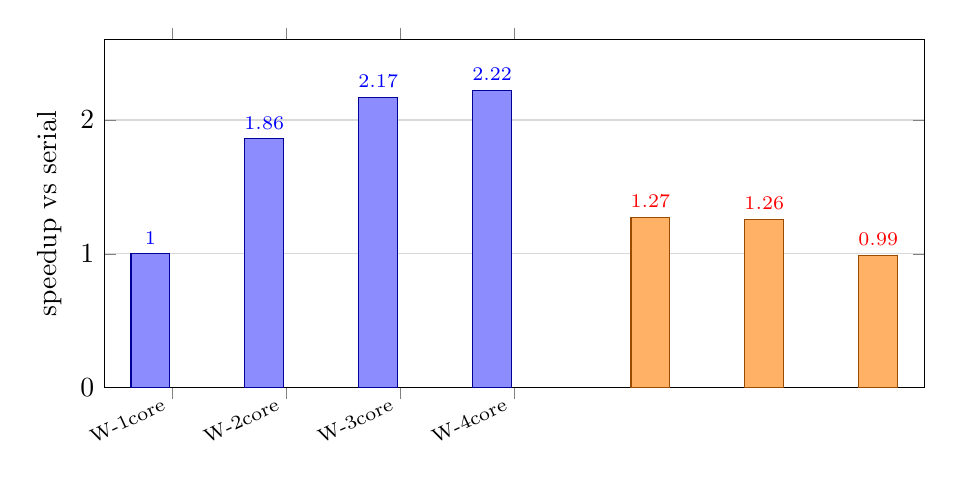
\begin{tikzpicture}
\begin{axis}[width=12cm,height=6cm,ybar,ymin=0,ymax=2.6,
  ylabel={speedup vs serial},
  symbolic x coords={W-1core,W-2core,W-3core,W-4core,S-2unit,S-8unit,S-4unit-old},
  xtick=data,x tick label style={rotate=25,anchor=east,font=\scriptsize},
  nodes near coords,nodes near coords style={font=\scriptsize},
  bar width=14pt,ymajorgrids,grid style={black!15}]
\addplot+[fill=blue!45,draw=blue!60!black] coordinates
  {(W-1core,1.00) (W-2core,1.86) (W-3core,2.17) (W-4core,2.22)};
\addplot+[fill=orange!60,draw=orange!60!black] coordinates
  {(S-2unit,1.27) (S-8unit,1.26) (S-4unit-old,0.99)};
\end{axis}
\end{tikzpicture}
\captionof{figure}{N-Queens $n=13$ の速度向上。青=ワーカーズ型、橙=対称SMP型。}
\end{center}

この表の対称SMP側は\textbf{核0がスケジューラに参加していない状態}の値である
（計器 \texttt{ran\_per\_core} の先頭が常に 0 ＝ 実質 3 コア）。
これは実装の穴であり、第\ref{sec:exp1}節で直した。\textbf{直したあとの
4 コア対 4 コアの比較は第\ref{sec:exp1}節を見よ}（ワーカーズ型 298.8 ms 対
対称SMP型 397 ms、差は 1.66 倍から \textbf{1.33 倍}へ縮んだ）。

\section{結果1b: 核0をスケジューラに参加させる（実験1）}\label{sec:exp1}

\subsection{原因は 2 段構えで、途中まで私の読みは誤っていた}
「核0が参加していない」ことは計器で分かっていたが、\textbf{どこで参加させるか}を
二度取り違えた。順に書く。実測でしか分からなかったからである。

\begin{enumerate}
\item \textbf{hook を置いた関数が呼ばれていなかった}。核0 は描画ループ
      \texttt{wm\_run()} に居ると考えて、そこへ引き取り口を置いた。しかし
      この板は HDMI が無く、\texttt{kernel\_main} は \texttt{shell\_main()} へ落ちる。
      \texttt{wm\_run()} は\textbf{呼び出し元が存在しない}。hook は一度も走っていなかった。
\item \textbf{移した先も回らなかった}。核0 の暇は \texttt{uart\_getc()} の
      RX 空回りだと考えて移したが、シリアルアダプタが TX$\to$RX ループバックのため
      RX FIFO がほとんど空にならない。計器 \texttt{poll\_calls} は HTTP 要求あたり
      約 1 回しか増えず、\texttt{poll\_hits} は 0 のままだった。
\item \textbf{正解は \texttt{proc\_preempt()}}。ここは 100\,Hz のタイマ IRQ から
      EOI 後に必ず呼ばれる。しかも既存の
      \texttt{if (!IS\_IDLE(currpid)) proc\_resched();} という判定こそが
      「核0 は idle だから何もしない」＝不参加の原因そのものだった。
\end{enumerate}

\noindent
なお \texttt{core\_hits}（AIPL メッセージをコア別に何通実行したか）を足して分かったのだが、
\textbf{AIPL の配布経路では核0 は最初から働いていた}。
\texttt{smpsched\_parallel} の「呼び手が最後の 1 単位を直接走らせる」ぶんが核0 で
実行されるからである。核0 不参加は \texttt{/smpsched}（N-Queens 駆動部）に固有の穴であって、
AIPL の配布経路の穴ではない。初稿の記述をここで訂正する。

\subsection{直した結果}

\begin{center}
\begin{tabular}{lrr}
\toprule
 & 修正前 (build 21:09:08) & \textbf{修正後 (build 21:37:48)} \\
\midrule
\texttt{ran\_per\_core}（4単位） & \textbf{0}/1/2/1 & \textbf{1/1/1/1} \\
N-Queens $n=13$ 最良 & 496 ms & \textbf{397 ms} \\
核0 が取った本数 \texttt{poll\_hits} & 0 & 13 \\
\bottomrule
\end{tabular}
\end{center}

\begin{center}
\begin{tabular}{lrr}
\toprule
\textbf{4 コア対 4 コア} & 時間 [ms] & 直列 660.1 ms からの速度向上 \\
\midrule
\textbf{ワーカーズ型 4コア} & \textbf{298.8} & \textbf{2.21} \\
対称SMP型（4単位, 最良） & 397 & 1.66 \\
\bottomrule
\end{tabular}
\end{center}

\noindent
\textbf{N-Queens ではワーカーズ型が 1.33 倍速い。}
修正前の 1.66 倍から縮んだので、\textbf{差の約半分は核0 の不参加という実装の穴が
作っていた}ことになる。残る 1.33 倍が方式そのものの差である。

\section{結果2: 通常の並列計算（負荷の性質による差）}

ワーカーズ型・4コア・同一起動。いずれも直列と並列で結果が一致（\texttt{agree=yes}）。

\begin{center}
\begin{tabular}{lrrr}
\toprule
負荷 & 直列 [ms] & 4コア [ms] & 速度向上 \\
\midrule
dining（独立卓・均一） & 95.59 & 23.92 & \textbf{4.00} \\
primes 30万（ほぼ均一） & 41.75 & 13.83 & \textbf{3.02} \\
nqueens $n{=}13$（木が不揃い） & 571.08 & 286.53 & 1.99 \\
fill 20万語（メモリ律速・短い） & 1.04 & 1.38 & 0.75 \\
\bottomrule
\end{tabular}
\end{center}

\begin{center}
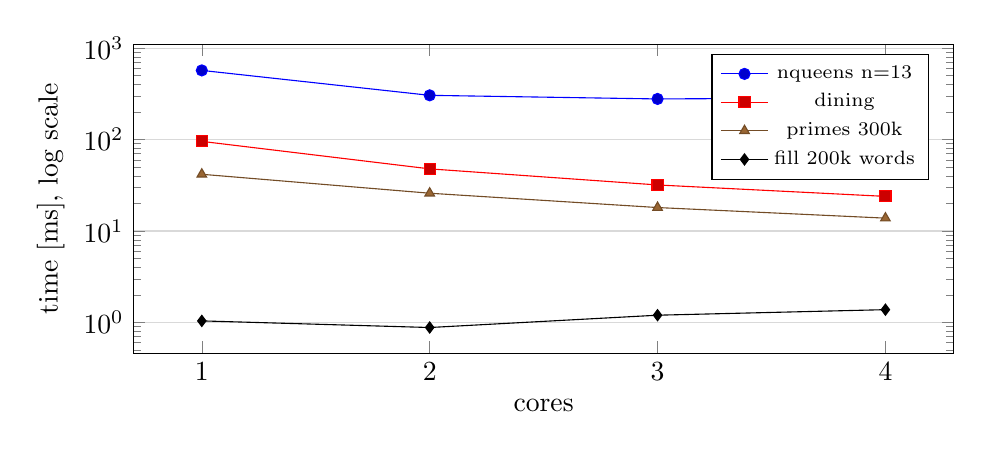
\begin{tikzpicture}
\begin{axis}[width=12cm,height=5.5cm,
  xlabel={cores},ylabel={time [ms], log scale},ymode=log,
  xtick={1,2,3,4},legend pos=north east,legend style={font=\scriptsize},
  ymajorgrids,grid style={black!15}]
\addplot+[mark=*] coordinates {(1,571.08)(2,304.79)(3,278.32)(4,286.53)};
\addlegendentry{nqueens n=13}
\addplot+[mark=square*] coordinates {(1,95.59)(2,47.84)(3,31.90)(4,23.92)};
\addlegendentry{dining}
\addplot+[mark=triangle*] coordinates {(1,41.75)(2,25.90)(3,18.06)(4,13.83)};
\addlegendentry{primes 300k}
\addplot+[mark=diamond*] coordinates {(1,1.04)(2,0.88)(3,1.20)(4,1.38)};
\addlegendentry{fill 200k words}
\end{axis}
\end{tikzpicture}
\captionof{figure}{ワーカーズ型のコア数掃引。均一な仕事は 4 コアぶん出る一方、
木が不揃いな nqueens は 3 コアで頭打ちになり、メモリ律速の fill は伸びない。}
\end{center}

\textbf{静的分割は、仕事が均一なら理想に近い}（dining で $4.00\times$）。
逆に不揃いだと一番重い区間を引いたコアの終了時刻が全体を決め、頭打ちになる。
これは静的分割の原理的な限界であり、対称SMP型が本来有利になりうる領域である。

\section{結果3: AIPL アクター並列（本命）}\label{sec:aipl}

\begin{center}\fbox{\parbox{0.93\textwidth}{\textbf{この節の数値についての断り。}
本節の測定は\textbf{駆動源を入れる前}に採ったもので、
第\ref{sec:flaw}節で述べたとおり\textbf{読み込み直後の 2 ラウンド（冷間始動の過渡）}
しか捉えていない。定常値は約 2 倍である。また\textbf{正誤を確認していない}。
したがって\textbf{絶対値は採用しない}。
一方、同じ条件で二方式を交互に測った\textbf{比}と、
コア別の実行数 \texttt{core\_hits} が示す\textbf{構造的な事実}は、
定常値で測り直した第\ref{sec:abc}節・第\ref{sec:boards3}節と整合しており、そのまま残す。}}\end{center}


\subsection{測り方}
AIPL 標本（\S\ref{sec:prog}）は 8 個の Worker が\textbf{同じ量}の計算をする。
宛先が互いに異なり \texttt{par\_safe}（WAIT も描画命令も含まない）なので、実行時系はこの
8 通を 1 つのバッチにまとめて配る。粒度（1 メッセージあたりのループ回数）を
1 から 200{,}000 まで 9 段階に振り、両方式で
\textbf{並列配布に費やした総時間 $us$} と\textbf{その間に配ったメッセージ数 $msgs$} を計器から読み、
$us/msgs$ を 1 メッセージあたりの費用とした。各点 2 回、再現性は $\pm 0.1\%$ 未満。

\subsection{測定値}

\begin{center}
\begin{tabular}{rrrr}
\toprule
粒度 [反復/msg] & ワーカーズ型 [$\mu$s/msg] & 対称SMP型 [$\mu$s/msg] & 比 \\
\midrule
1        & 3.56 & 5.31 & \textbf{1.49} \\
10       & 8.94 & 11.69 & 1.31 \\
50       & 36.72 & 39.63 & 1.08 \\
200      & 141.91 & 144.81 & 1.02 \\
1{,}000    & 699.50 & 704.09 & 1.01 \\
5{,}000    & 3{,}487.06 & 3{,}505.88 & 1.005 \\
20{,}000   & 13{,}954.62 & 14{,}005.00 & 1.004 \\
100{,}000  & 69{,}764.09 & 70{,}009.50 & 1.004 \\
200{,}000  & 139{,}695.69 & 140{,}007.62 & 1.002 \\
\bottomrule
\end{tabular}
\end{center}

\begin{center}
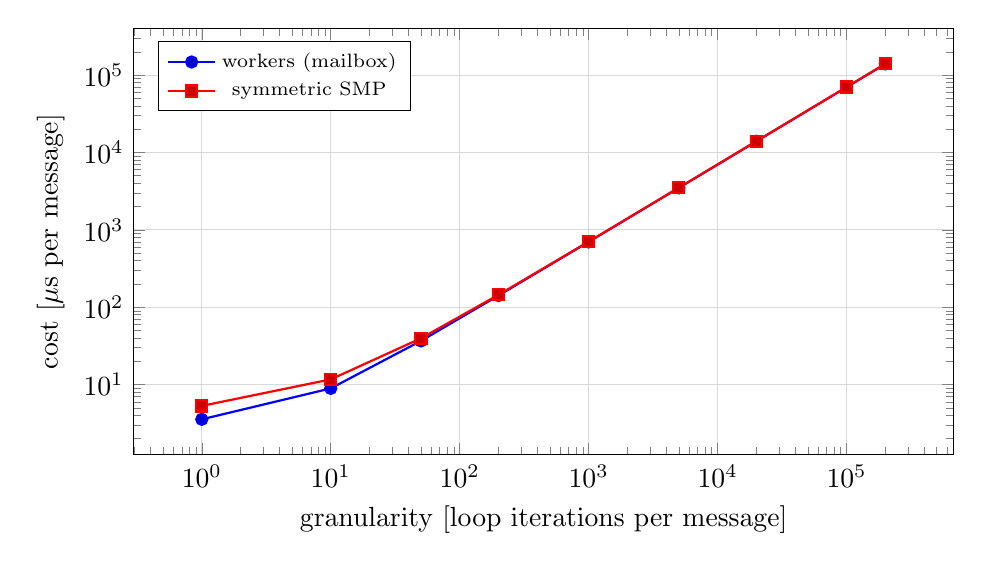
\begin{tikzpicture}
\begin{axis}[width=12cm,height=7cm,xmode=log,ymode=log,
  xlabel={granularity [loop iterations per message]},
  ylabel={cost [$\mu$s per message]},
  legend pos=north west,legend style={font=\scriptsize},
  ymajorgrids,xmajorgrids,grid style={black!15}]
\addplot+[mark=*,thick] coordinates \aiplW;   \addlegendentry{workers (mailbox)}
\addplot+[mark=square*,thick] coordinates \aiplS; \addlegendentry{symmetric SMP}
\end{axis}
\end{tikzpicture}
\captionof{figure}{AIPL のメッセージ 1 通あたりの費用。粒度が大きい領域では
両者は重なる（本体の実行が支配的）。細かい領域で分かれる。}
\end{center}

\begin{center}
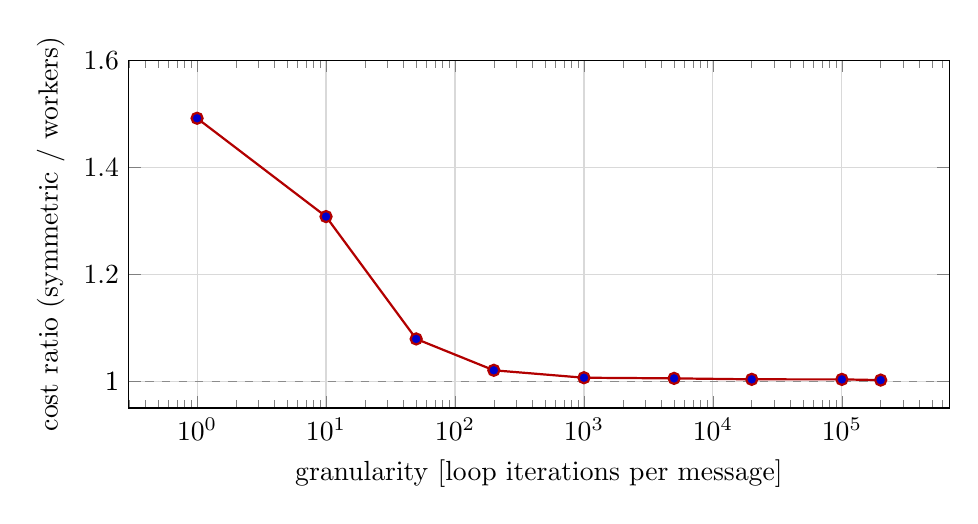
\begin{tikzpicture}
\begin{axis}[width=12cm,height=6cm,xmode=log,
  xlabel={granularity [loop iterations per message]},
  ylabel={cost ratio (symmetric / workers)},
  ymin=0.95,ymax=1.6,ymajorgrids,xmajorgrids,grid style={black!15},
  extra y ticks={1.0},extra y tick style={grid=major,grid style={black!45,dashed}}]
\addplot+[mark=*,thick,color=red!70!black] coordinates \aiplRatio;
\end{axis}
\end{tikzpicture}
\captionof{figure}{同じ仕事に対する費用の比。粒度が細かいほどワーカーズ型が有利になり、
粒度 1 反復では 1.49 倍の差がつく。粒度 200 反復（$\simeq 140\,\mu$s の仕事）を超えると
差は 2\% 以下に埋もれる。}
\end{center}

\subsection{配布コストの分離}

粒度が小さい領域（$\le 1{,}000$）で $us/msg = a + b\times$粒度 に当てはめると:

\begin{center}
\begin{tabular}{lrr}
\toprule
 & 配布コスト $a$ [$\mu$s/msg] & 傾き $b$ [ns/反復/msg] \\
\midrule
ワーカーズ型 & \textbf{2.28} & 697.2 \\
対称SMP型 & \textbf{4.71} & 699.4 \\
\midrule
差 & \textbf{2.43}（\textbf{2.06 倍}） & 0.3\%（一致） \\
\bottomrule
\end{tabular}
\end{center}

\begin{center}
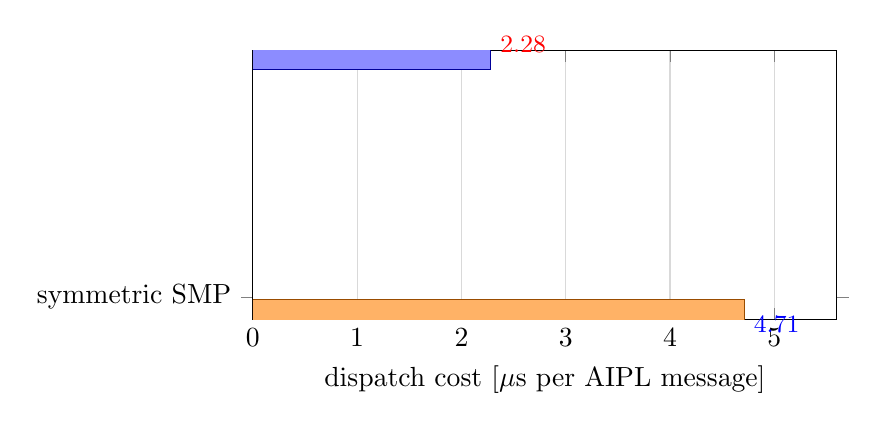
\begin{tikzpicture}
\begin{axis}[width=9cm,height=5cm,xbar,xmin=0,
  xlabel={dispatch cost [$\mu$s per AIPL message]},
  symbolic y coords={symmetricSMP,workers},ytick=data,
  yticklabels={symmetric SMP,workers (mailbox)},
  nodes near coords,nodes near coords style={font=\small},
  bar width=18pt,xmajorgrids,grid style={black!15},xmax=5.6]
\addplot+[fill=orange!60,draw=orange!60!black] coordinates {(4.71,symmetricSMP)};
\addplot+[fill=blue!45,draw=blue!60!black] coordinates {(2.28,workers)};
\end{axis}
\end{tikzpicture}
\captionof{figure}{AIPL メッセージ 1 通を配るのに要する費用。本体の実行時間は含まない。}
\end{center}

\paragraph{傾き $b$ の読み方（訂正）。}
$b$ を「解釈器 1 反復の所要時間」と読んではならない。測っているのは
\emph{バッチ全体の壁時計時間をバッチ内メッセージ数で割った値}なので、
バッチが 4 コアで同時に走るぶん $b$ には $1/4$ が掛かっている。
すなわち解釈器の素の速度は $b\times 4 \simeq 2.79\,\mu\mathrm{s}$/反復である。
（この $2.79\,\mu\mathrm{s}$ は第\ref{sec:abc}節で独立に検証される。）
初稿ではここを取り違えて「バッチが直列に走っている」と述べたが、
第\ref{sec:exp2}節のバッチ長掃引がそれを否定した。

\textbf{$b$ が両方式で一致している}ことが重要である。本体の実行速度は同じなのだから、
$a$ の差は\textbf{配布機構そのものの費用}である。ワーカーズ型は 1 バッチにつき
郵便箱への書き込みと \texttt{SEV} 一回で済み、その費用がバッチ内の 8 通に薄まる。
対称SMP型は 1 単位ごとにプロセスを作り、共有キューのロックを取り、文脈を切り替える。


\section{結果4: バッチ長と並列度（実験2）}\label{sec:exp2}

\begin{center}\fbox{\parbox{0.93\textwidth}{\textbf{この節の数値についての断り。}
本節の測定は\textbf{駆動源を入れる前}に採ったもので、
第\ref{sec:flaw}節で述べたとおり\textbf{読み込み直後の 2 ラウンド（冷間始動の過渡）}
しか捉えていない。定常値は約 2 倍である。また\textbf{正誤を確認していない}。
したがって\textbf{絶対値は採用しない}。
一方、同じ条件で二方式を交互に測った\textbf{比}と、
コア別の実行数 \texttt{core\_hits} が示す\textbf{構造的な事実}は、
定常値で測り直した第\ref{sec:abc}節・第\ref{sec:boards3}節と整合しており、そのまま残す。}}\end{center}


前節の粒度掃引はバッチ長を 8 に固定していた。バッチ長そのものを振ると、
\textbf{AIPL のアクター・バッチが本当に 4 コアで同時に走っているか}が分かる。
標本は \texttt{AiplP$n$.abcl}（アクター $n$ 個・各 1{,}000 反復・粒度は全て同じ）。

\begin{center}
\begin{tabular}{lrrrrrrr}
\toprule
バッチ長 & msgs & 巡回数 & \multicolumn{3}{c}{1 メッセージあたり [$\mu$s]} & \multicolumn{2}{c}{1 巡 [$\mu$s]} \\
\cmidrule(lr){4-6}\cmidrule(lr){7-8}
 & & & W & S & S/W & W & S \\
\midrule
2+2 & 4 & 2 & 1072.5 & 1093.0 & 1.019 & 2145 & 2186 \\%
4+4 & 8 & 2 & 686.0 & 690.9 & 1.007 & 2744 & 2764 \\%
8+8 & 16 & 4 & 699.1 & 705.7 & 1.009 & 2796 & 2823 \\%
16+16 & 32 & 8 & 740.3 & 746.8 & 1.009 & 2961 & 2987 \\%
32+23 & 55 & 14 & 581.7 & 590.3 & 1.015 & 2285 & 2319 \\
\bottomrule
\end{tabular}
\end{center}

\noindent
「巡回数」は $\sum \lceil \text{バッチ長}/4 \rceil$、すなわち 4 コアで何巡すれば
そのバッチを配り終えるかである。W = ワーカーズ型、S = 対称SMP型。

\begin{center}
\begin{tikzpicture}
\begin{axis}[width=11cm,height=6cm,xmode=log,log basis x=2,
  xlabel={バッチ長（同時に発射されたメッセージ数）},
  ylabel={1 メッセージあたり [$\mu$s]},
  ymin=500,ymax=1150,legend pos=north east,
  xmajorgrids,ymajorgrids,grid style={black!15}]
\addplot+[mark=*,thick] coordinates \batW;   \addlegendentry{workers (mailbox)}
\addplot+[mark=square*,thick] coordinates \batS; \addlegendentry{symmetric SMP}
\end{axis}
\end{tikzpicture}
\captionof{figure}{バッチ長を変えたときの 1 メッセージあたりの費用。
バッチ長 2（コア数 4 に満たない）では約 2 倍高く、4 以上でほぼ一定になる。}
\end{center}

\paragraph{読み取れること。}
\begin{enumerate}
\item \textbf{バッチはコア数まで並列に走っている}。バッチ長 2 では 1{,}072$\,\mu$s/msg、
      4 では 686$\,\mu$s/msg。半分に落ちるのは、長さ 2 のバッチが 4 コアのうち
      2 コアしか使えていないからである。\textbf{直列に走っているなら
      バッチ長を変えても $\mu$s/msg は変わらないはずで、この落ち込みが並列の証拠になる。}
\item 「1 巡」の欄（1{,}000 反復を全コア同時に走らせた所要時間）は
      2{,}100$\sim$3{,}000$\,\mu$s にほぼ収まる。$\Rightarrow$ 解釈器 1 反復
      $\simeq 2.8\,\mu\mathrm{s}$。前節の傾き $b\simeq 700\,$ns の 4 倍で、辻褄が合う。
\item \textbf{方式差はどのバッチ長でもほぼ一定}（S/W $= 1.007\sim1.019$）。
      この粒度（1{,}000 反復 $\simeq 2.8\,$ms）では配布コストは埋もれる。
      方式差が効くのは第\ref{sec:aipl}節で見たとおり\textbf{粒度が小さいとき}である。
\end{enumerate}

\noindent
（バッチ長 32 の標本は実測でバッチが $32+23$ に割れており、他の行と同列には読めない。
再測が必要な行として残す。）

\section{結果5--8（改訂）: 定常値で測り直した実験A・B・C}\label{sec:abc}

\textbf{第\ref{sec:flaw}節で述べた 3 つの穴を直したうえで、実験A・B・C を測り直した。}
以下はすべて\textbf{暖機を捨てた定常値}であり、\textbf{全点 \texttt{ng=0}}
（各ラウンドの合計が検算に通ったこと）を確認してある。
方式はワーカーズ型（郵便箱・静的分割）。対称SMP型については第\ref{sec:symbroken}節を見よ。

\subsection{実験A: 交差点はどこか（ばらつき比の掃引）}
総仕事量を 128{,}000 反復に固定し、8 アクターへの配分のばらつき比だけを振る。

\begin{center}
\begin{tabular}{rrrrrr}
\toprule
比 & \multicolumn{2}{c}{Pi 5 (A76)} & \multicolumn{2}{c}{Pi 4 (A72)} & 予測比 \\
\cmidrule(lr){2-3}\cmidrule(lr){4-5}
 & ms/batch & 比 & ms/batch & 比 & (静的 makespan) \\
\midrule
1 & 186.0 & 1.00 & 253.8 & 1.00 & 1.00 \\
2 & 248.1 & 1.33 & --- & --- & 1.32 \\
4 & 308.7 & 1.66 & 412.1 & 1.62 & 1.65 \\
8 & 365.1 & 1.96 & --- & --- & 1.98 \\
16 & 415.7 & 2.23 & 557.3 & 2.20 & 2.28 \\
32 & 460.1 & 2.47 & --- & --- & 2.57 \\
64 & 498.8 & 2.68 & 671.3 & 2.64 & 2.81 \\
128 & 534.3 & \textbf{2.87} & 715.2 & \textbf{2.82} & \textbf{3.01} \\
\bottomrule
\end{tabular}
\end{center}

\noindent
\textbf{A76 と A72 で比の曲線がほぼ一致する}（最遠点で 2.87 対 2.82）。
静的分割の makespan モデルは\textbf{アーキテクチャに依らない}性質である。
絶対値は Pi 5 のほうが 1.2$\sim$1.4 倍速い。

\subsection{実験B: 細かく割れば静的分割は救えるか}
同じ重み集合（$1..M$ を正規化、合計 128{,}000 反復）を、
\textbf{散らした場合 B1}（ビット反転順）と\textbf{後ろに固めた場合 B2}（単調増加）で比べる。

\begin{center}
\begin{tabular}{lrrrrr}
\toprule
 & \multicolumn{2}{c}{$M=4$} & \multicolumn{2}{c}{$M=8$} & $M=16$ \\
\midrule
Pi 5 \ B1 散らす & \multicolumn{2}{r}{301.5 ms} & \multicolumn{2}{r}{255.5 ms} & \textbf{235.3 ms} \\
Pi 5 \ B2 固める & \multicolumn{2}{r}{301.5 ms} & \multicolumn{2}{r}{322.6 ms} & \textbf{349.4 ms} \\
Pi 4 \ B1 散らす & \multicolumn{2}{r}{408.9 ms} & \multicolumn{2}{r}{339.1 ms} & \textbf{300.2 ms} \\
Pi 4 \ B2 固める & \multicolumn{2}{r}{410.6 ms} & \multicolumn{2}{r}{424.6 ms} & \textbf{434.7 ms} \\
\bottomrule
\end{tabular}
\end{center}

\noindent
\textbf{両板で同じ向きに分かれた。} 郵便箱は区間を\textbf{連続}に 4 等分するので、
重い仕事が散らばっていれば $M$ を増やすほど平均化されて速くなり
（Pi 5: $301.5 \to 235.3$、Pi 4: $408.9 \to 300.2$）、
固まっていれば同じコアに集まり続けて\textbf{遅くなる}
（Pi 5: $301.5 \to 349.4$、Pi 4: $410.6 \to 434.7$）。

\textbf{処方は「共有 ready キューへ移れ」ではない。}
\textbf{多めに分割し、重い仕事を隣り合わせにするな} ---- 郵便箱方式のまま実行できる。

\subsection{実験C: 4 コアで 4 倍は出ない}
仕事を完全に等量（1 通 32{,}000 反復）にしたまま、バッチ長で使用コア数だけを変える。

\begin{center}
\begin{tabular}{rrrrr}
\toprule
使用コア & \multicolumn{2}{c}{Pi 5 (A76)} & \multicolumn{2}{c}{Pi 4 (A72)} \\
\cmidrule(lr){2-3}\cmidrule(lr){4-5}
 & ms/batch & 1 反復 & ms/batch & 1 反復 \\
\midrule
2 & 145.3 & 4.54 $\mu$s & 215.3 & 6.73 $\mu$s \\
3 & 164.1 & 5.13 $\mu$s & 232.8 & 7.28 $\mu$s \\
4 & 185.5 & \textbf{5.80} $\mu$s & 255.0 & \textbf{7.97} $\mu$s \\
\midrule
2$\to$4 コアの劣化 & \multicolumn{2}{c}{\textbf{$+27.7\%$}} & \multicolumn{2}{c}{\textbf{$+18.4\%$}} \\
実効スループット & \multicolumn{2}{c}{1.57$\times$（理想 2.00）} & \multicolumn{2}{c}{1.69$\times$（理想 2.00）} \\
\bottomrule
\end{tabular}
\end{center}

\noindent
\textbf{分割の不均等はゼロなのに、コアを増やすと 1 反復の所要が伸びる。}
両板とも D-cache を切って走っているので、すべてのメモリ参照がバスに出る。
\textbf{A72 のほうが劣化が小さい}（$+18.4\%$ 対 $+27.7\%$）のは、
素の 1 反復が遅い（6.73 対 4.54\,$\mu$s）ぶんメモリ帯域への要求が緩いためと読める。
N-Queens が 4 コアで $2.2\times$ 止まりだった主因はここにある。

\subsection{不揃いな仕事（旧・実験3）}
\texttt{AiplUneven}（8 アクター、$1{,}000\cdot 2^k$ 反復、合計 255{,}000）の定常値は
Pi 5 が 1{,}065.5 ms/batch、Pi 4 が 1{,}424.6 ms/batch。
\textbf{対称SMP型との比較は、対称側が正しく動かないため取れていない}
（第\ref{sec:symbroken}節）。初稿にあった「対称SMP型が 1.25 倍速い」は撤回する
（第\ref{sec:retract}節）。

\section{撤回: 「不揃いな仕事では対称SMP型が 1.25 倍速い」}\label{sec:retract}

初稿の第9節（実験3）で、\texttt{AiplUneven} について
\textbf{対称SMP型が 1.25 倍速い（403.1 ms 対 505.1 ms）}と報告した。
\textbf{これを撤回する。} 理由は 2 つある。

\begin{enumerate}
\item \textbf{定常値ではなかった。} その測定は駆動源が無い状態で採られており、
      実際には\textbf{読み込み直後の 2 ラウンド}しか走っていない。
      同じ標本の定常値は Pi 5 で 1{,}065.5 ms/batch であり、約 2 倍である。
\item \textbf{正誤を確認していなかった。} 検算計器を入れて測り直すと、
      \textbf{対称SMP型の AIPL 経路は誤った答えを返す回がある}（第\ref{sec:symbroken}節）。
\end{enumerate}

\noindent
\textbf{計算が誤っているなら、速さに意味は無い。}
「静的分割は最も重い区間に律速される」という理論的な指摘そのものは依然として正しく、
実験Bはその影響を実測している。しかし\textbf{この実装で
「対称SMP型のほうが速い」を実測できたとは言えない。}


\section{結果9: 三板での追試（Pi 4 / Pi 3）}\label{sec:boards3}

Pi 5 で得た「分割の仕方が効く」という結論を、別アーキテクチャで確かめる。
Pi 4（Cortex-A72）と Pi 3（Cortex-A53）には対称SMPスケジューラは無いので、
ここで比べるのは\textbf{ワーカーズ型（郵便箱・静的分割）における分割の仕方}である。

\subsection{N-Queens $n=13$}

\begin{center}
\begin{tabular}{lrrr}
\toprule
コア & Pi 5 (A76) & Pi 4 (A72) & Pi 3 (A53) \\
\midrule
1 & 660.1 ms (1.00$\times$) & 1401.3 ms (1.00$\times$) & 1426.1 ms (1.00$\times$) \\
2 & 355.8 ms (1.85$\times$) & 959.3 ms (1.46$\times$) & 789.0 ms (1.81$\times$) \\
3 & 306.0 ms (2.16$\times$) & 859.0 ms (1.63$\times$) & 641.6 ms (2.22$\times$) \\
4 & \textbf{298.8 ms (2.21}$\times$\textbf{)} & \textbf{847.9 ms (1.65}$\times$\textbf{)}
  & \textbf{517.4 ms (2.76}$\times$\textbf{)} \\
\bottomrule
\end{tabular}
\end{center}
\begin{center}
\begin{tikzpicture}
\begin{axis}[width=11cm,height=5.6cm,xlabel={コア数},ylabel={速度向上},
  xtick={1,2,3,4},ymin=0.9,ymax=3.0,legend pos=north west,
  xmajorgrids,ymajorgrids,grid style={black!15}]
\addplot+[mark=*,thick] coordinates {(1,1.00)(2,1.85)(3,2.16)(4,2.21)};
  \addlegendentry{Pi 5 (A76)}
\addplot+[mark=triangle*,thick] coordinates {(1,1.00)(2,1.46)(3,1.63)(4,1.65)};
  \addlegendentry{Pi 4 (A72)}
\addplot+[mark=square*,thick] coordinates {(1,1.00)(2,1.81)(3,2.22)(4,2.76)};
  \addlegendentry{Pi 3 (A53)}
\addplot[dashed,black,domain=1:4,samples=2] {3.01};
  \addlegendentry{均一負荷での天井 3.01}
\end{axis}
\end{tikzpicture}
\captionof{figure}{N-Queens $n=13$ の速度向上（各 3 回の中央値、ばらつきは全点 0.1\% 未満）。
\textbf{Pi 4 は 3 コアで頭打ちになる}のに対し、Pi 3 は 4 コア目でも伸びる。}
\end{center}

\noindent
\textbf{Pi 3 と Pi 4 は直列がほぼ同じ}（1426 対 1401 ms）\textbf{なのに、4 コアでは
Pi 3 が 1.6 倍速い}。素直に読めば「A53 のほうが並列に強い」となるが、それは誤りである。
なお \textbf{Pi 4 は 3 コアで頭打ちになる}（$1.63\times \to 1.65\times$）。
連続分割で重い列が同じコアに固まると、コアを足しても効かなくなる
---- 第\ref{sec:abc}節と同じ形である。

\subsection{均一な負荷なら三板とも同じ}

分割の不均等がほとんど無い負荷（\texttt{primes}, $n=300{,}000$）で測り直す。

\begin{center}
\begin{tabular}{lrr}
\toprule
コア & Pi 4 & Pi 3 \\
\midrule
1 & 0.99$\times$ & 1.00$\times$ \\
2 & 1.61$\times$ & 1.61$\times$ \\
3 & 2.31$\times$ & 2.31$\times$ \\
4 & \textbf{3.01}$\times$ & \textbf{3.01}$\times$ \\
\bottomrule
\end{tabular}
\end{center}

\noindent
\textbf{曲線が完全に一致した}（Pi 5 の \texttt{primes} も 3.02$\times$）。
したがって N-Queens の差はハードウェアの差ではなく、
\textbf{各カーネルが N-Queens をどう分割しているか}の差である。

\subsection{分割の仕方だけを変える}

Pi 4 は \texttt{/bench?il=} で分割を選べる（各 2 回、再現性あり）。

\begin{center}
\begin{tabular}{lrr}
\toprule
分割 & 4 コア [ms] & 速度向上 \\
\midrule
\texttt{il=0} 連続 4 等分 & 847.6 / 847.3 & 1.64$\times$ \\
\texttt{il=1} ストライド（第1行） & 811.1 / 811.1 & 1.72$\times$ \\
\texttt{il=2} ストライド（第2行・Pi 3 と同じ方式） & \textbf{774.3 / 774.4} & \textbf{1.81}$\times$ \\
\bottomrule
\end{tabular}
\end{center}

\noindent
\textbf{スケジューラを一切変えず、分割の仕方を変えるだけで $+10\%$。}
第\ref{sec:abc}節（重い仕事を散らせば静的分割は救える）の、
\textbf{実機・別アーキテクチャでの追認}である。
なお Pi 3 は \texttt{il=} を受け付けず既定の分割ひとつだけだが、それで 2.75$\times$ 出る。
Pi 4 の \texttt{il=2} が本当に Pi 3 と同じ分割なら 1.81$\times$ 対 2.75$\times$ の差が残るので、
別要因（D-cache の扱い、L2 の共有の仕方）を疑う必要がある。ここは未解決である。

\subsection{Pi 3 は「アクター＝スレッド」という別の方式だった}
Pi 3 に AIPL のバッチ配布を移植しようとして、\textbf{移植すべきものが無い}と分かった。
Pi 3 の AIPL アクターは\textbf{Xinu スレッド＋メールボックス}である
（\texttt{objects[i].tid}（\texttt{tid\_typ}）、\texttt{semcreate(0)}、
アクターごとの consumer スレッド）。バイトコード VM はそのスレッド機構の上に載っており
（VM クラスは \texttt{VM\_CLASS\_BASE=200} 以降の class\_id を取る）、
「メッセージを束ねてコアへ配る」段階が存在しない。
\textbf{Pi 3 は最初からアクター＝共有 ready キュー上のスレッド}であり、
構造としては対称SMP型に相当する。

Pi 3 にも同じ計器（\texttt{/avm-par}, \texttt{ok}/\texttt{ng}, \texttt{core\_hits}）と
駆動源（\texttt{/avm-run}）を移植して測ったところ、次の 2 つが分かった。

\paragraph{(1) 1 通も他コアへ配られない。}
\texttt{core\_hits} は常に $N/0/0/0$ である ---- 4 アクターでも 16 アクターでも、
すべてのメッセージが核0 で実行される。アクターがスレッドであっても、
\textbf{この Xinu はスレッドをコア間に分散しない}。多コアを使うのは
\texttt{smp\_parallel\_sum} を明示的に呼ぶ経路（\texttt{/bench}）だけである。
同じ標本で Pi 4 / Pi 5 は $N/N/N/N$ と均等に散る。

\paragraph{(2) 計算の重いアクターを 8 個載せると系が止まった。}
\texttt{AiplP8} を載せた直後から HTTP がまったく応答しなくなった
（\texttt{ping} は 100\% 通るのでネットワークは生存）。原因は
VM アクターの優先度が \texttt{default: INITPRIO(20)} で
\textbf{Web サーバ（\texttt{webactor\_server}、同じく INITPRIO）と同値}だったことである。
VM アクターだけ \texttt{INITPRIO-5} に下げて解消した。
\textbf{アクター＝データ方式では VM が協調的に tick するので、
優先度の設計を誤っても系は止まらない。}

\paragraph{定量比較は保留する。}
Pi 3 の \texttt{us} は使えない（複数のディスパッチが同時に計時中になり、
壁時計の区間が重なって 2 秒の窓に 21.4 秒を計上する）。
共通の物差しは \texttt{ok} だが、\textbf{Pi 3 は暖機後 11 ラウンドで止まる}という
未解決の問題があり（第\ref{sec:open}節）、スループットを Pi 4 と並べるのは時期尚早である。
確実に言えるのは上の (1) と (2) の\textbf{構造的な事実}に限る。

\subsection{4 コアで 4 倍は出ない、も三板に共通}
均一な負荷でも 4 コアで 3.01$\times$（Pi 5 も 3.02$\times$）。
分割の不均等がゼロでもここが天井であることは、第\ref{sec:abc}節と整合する。

\section{結果10: Pi 4 にも同じ例外復帰の穴があった}\label{sec:pi4bug}

第\ref{sec:bug}節で Pi 5 に見つけた穴（例外エントリが \texttt{ELR\_EL1}/\texttt{SPSR\_EL1} を
退避しない）が、\textbf{Pi 4 にもそのまま存在した}。

\begin{itemize}
\item \texttt{irq\_dispatch\_c} $\to$ \texttt{proc\_preempt()} $\to$ \texttt{proc\_resched()}
      $\to$ \textbf{割り込み区間の中で \texttt{ctxsw}}
\item \texttt{irq\_entry} は x0--x30 と \textbf{q0--q31 まで}退避するのに
      \texttt{ELR\_EL1}/\texttt{SPSR\_EL1} は退避しない
\item その場のコメント自身が「\texttt{irq\_dispatch\_c} は ctxsw を呼びうるので
      割り込まれた側の FP 状態は生き延びねばならない」と書いている。
      \textbf{同じ理屈が ELR/SPSR にも当てはまるのに抜けていた。}
\end{itemize}

\subsection{計器そのものを先に検証する}
最初の測定は \texttt{mismatch=0}、つまり\textbf{穴が無いように見えた}。
しかしそれは \textbf{Pi 4 が先取り(preemption)を既定で切っている}ためで、
\textbf{危険が起こり得ない状態を測っていた}のである。

\begin{center}
\begin{tabular}{ll}
\toprule
\texttt{/netpreempt} & \texttt{net\_preempt=off}（既定） \\
\texttt{/rtos-jitter preempt=0} & \texttt{pp\_calls=1296 off=1296 fired=0} ← 一度も発火しない \\
\texttt{/rtos-jitter preempt=1} & \texttt{pp\_calls=605 off=0 fired=605} ← 発火する \\
\bottomrule
\end{tabular}
\end{center}

\subsection{同じ起動のまま A/B を取る}
\texttt{/elrfix?on=0|1} で復帰時の書き戻しを実行時に切り替えられるようにし、
\texttt{/preempttest?procs=\&n=} で答えの決まった計算（積・和・剰余のみ、メモリを持たない）を
複数プロセスで同時に回して基準値と突き合わせた。先取りは ON。

\begin{center}
\begin{tabular}{lll}
\toprule
プロセス数 & 修正なし \texttt{elr\_restore\_on=0} & 修正あり \texttt{=1} \\
\midrule
2 & \texttt{991055 906373} → \textbf{mismatch 2/2} & 全て 480003 → \textbf{0} \\
4 & \texttt{428433 258890 504716 480003} → \textbf{3/4} & 全て 480003 → \textbf{0} \\
8 & 8 個すべて相異なる値 → \textbf{8/8} & 全て 480003 → \textbf{0} \\
\bottomrule
\end{tabular}
\end{center}

\noindent
期待値は 480003。\textbf{先取りが入った瞬間に、修正なしでは答えが全部狂う。}
修正あり側は N-Queens も 1397.2 / 960.8 / 847.8 ms・解 73712・\texttt{agree = yes} と
焼く前に一致し、退行は無い。

\subsection{Pi 3 に同じ穴は無い ---- ARM32 の実装は正しかった}
Pi 3 の実機カーネルは \texttt{kernel7.img}、すなわち \textbf{ARMv7 (32 bit)} で、
\texttt{xinu-rpi4}/\texttt{xinu-rpi5} とは別系統（classic Embedded Xinu）である。
AArch64 の \texttt{ELR\_EL1}/\texttt{SPSR\_EL1} に相当するのはバンクされた
\texttt{LR\_irq}/\texttt{SPSR\_irq} で、その IRQ 入口はこうなっている:

\begin{lstlisting}
    sub  lr, lr, #4
    srsdb #ARM_MODE_SYS!     /* SPSR_irq と LR_irq を **SYS スタック** へ積む */
    cpsid if, #ARM_MODE_SYS  /* = 割り込まれたスレッド自身のスタック          */
    push {r0-r4, r12, lr}
    bl   dispatch            /* この中で clkhandler -> resched() が起こりうる */
    pop  {r0-r4, r12, lr}
    rfeia sp!                /* 自分のスタックから PC と CPSR を戻す          */
\end{lstlisting}

\noindent
\textbf{復帰状態を「割り込まれたスレッド自身のスタック」に積んでいる}ので、
\texttt{dispatch()} の中で文脈が切り替わっても、各スレッドは自分の復帰状態を持って戻る。
\texttt{clkhandler.c} は実際に割り込み中に \texttt{resched()} を呼ぶが、それでも安全である。

\textbf{つまり AArch64 版（rpi4/rpi5）は、ARM32 版が正しくやっていたことを
再実装の際に落としていた。} Pi 3 は対象外であり、焼き直しも要らない。

\subsection{三板の測定状況}

\begin{center}
\begin{tabular}{llll}
\toprule
実験 & Pi 5 & Pi 4 & Pi 3 \\
\midrule
N-Queens コア 1--4 & 済 & 済 & 済 \\
均一負荷 \texttt{primes} コア 1--4 & 済 & 済 & 済 \\
分割の仕方 \texttt{il=} & 口あり & 済 & 対象外（受け付けない） \\
ELR/SPSR の穴 & 済（発見・修正） & 済（実証・修正） & \textbf{対象外}（ARM32 で元から正しい） \\
\texttt{dining} / \texttt{fill} & 済 & 済 & 未対応 \\
AIPL 実験 A/B/C & 済 & \textbf{未実装} & \textbf{未実装} \\
対称SMP型 & 済 & \textbf{未移植} & \textbf{未移植} \\
実験1（核0 の参加） & 済 & 対象外 & 対象外 \\
\bottomrule
\end{tabular}
\end{center}

\noindent
Pi 3 / Pi 4 で残っているのは \textbf{AIPL のアクター並列}と\textbf{対称SMP型}の 2 つだけで、
どちらも機構そのものが無いため、実装（移植）が先である。
Pi 3 は classic Embedded Xinu の系統なので、Pi 5 からの移植は Pi 4 より重い。


\section{対称SMP型の AIPL 経路は動かなかった ---- その診断}\label{sec:symbroken}

検算計器を入れて対称SMP型で AIPL を測ると、\textbf{壊れていることが直ちに分かった}。

\subsection{症状}
\begin{center}
\begin{tabular}{lll}
\toprule
標本 & 結果 & \texttt{core\_hits} \\
\midrule
\texttt{AiplSpread1} & \texttt{ok=37} \textbf{\texttt{ng=28}} & 178/128/126/128（偏り）\\
\texttt{AiplSpread4} & \texttt{ok=2} \textbf{\texttt{ng=78}} & 219/186/116/115 \\
\texttt{AiplEq4} & \texttt{ok=0}、1 バッチに 4{,}150 ms & 1/1/1/1 \\
\bottomrule
\end{tabular}
\end{center}

同じ標本を 3 回繰り返すと\textbf{回ごとに挙動が変わる} ---- 正しく速く走る回、
まったく進まない回、1 バッチに 4 秒かかる回が混ざる。
さらに\textbf{測定中に板がネットワークごと停止した}（\texttt{ping} も通らない）。
一方 \textbf{N-Queens の対称経路（\texttt{/smpsched}）は正しいまま}であり
（\texttt{solutions=73712}, \texttt{ran\_per\_core=1/1/1/1}, 411 ms）、
壊れているのは \textbf{AIPL のバッチ配布に固有}である。

\subsection{外れた仮説1: 控えの添字の競合}
\texttt{par\_send} / \texttt{par\_spawn} はコアごとの控えを第3引数で選ぶので、
同時に走る実行のあいだで一意でなければならない。郵便箱方式は 1 コア 1 単位に固定するが、
対称方式では単位が普通のプロセスなので、先取りで同じコアに別の単位が載りうる ----
と考えて、添字を\textbf{単位番号}に変えた。\textbf{直らなかった。}

\subsection{外れた仮説2 → 部分的に当たり: 静的スタックの再利用}
\texttt{sp\_task} は \texttt{sp\_done++} したあとも\textbf{自分のスタックの上で}
\texttt{proc\_exit()} を実行し続ける。駆動側は \texttt{sp\_done} を見た瞬間に戻るので、
次の呼び出しが同じ静的スタックへ新しい文脈を書き込む。
AIPL は毎秒数百回ここを通るので必ず踏み、N-Queens は HTTP 要求ごとに 1 回しか
通らないので踏まない ---- 観測と一致する。

スタックを\textbf{世代}で回して（同じ領域の再利用まで 4 バッチ挟む）測り直すと:

\begin{center}
\begin{tabular}{lrr}
\toprule
 & 世代化なし & \textbf{世代化あり} \\
\midrule
\texttt{ng} & 28$\sim$78 & \textbf{0$\sim$1} \\
\texttt{core\_hits} & 178/128/126/128 & \textbf{22/22/22/22} \\
\texttt{reuse}（再利用時にまだ \texttt{PR\_FREE} でなかった回数） & --- & \textbf{1$\sim$2} \\
\bottomrule
\end{tabular}
\end{center}

\noindent
\textbf{\texttt{reuse} が 0 でないことが、この危険が実際に起きている証拠}である。
世代化で誤答は激減し、配り分けの偏りも消えた。\textbf{ただし主因ではなかった}
---- 1 バッチ 4{,}150 ms という異常は残った。

\subsection{当たり: 呼び手が自分で計算していること}
時間の行き先を分解する計器を入れたところ、答えが一目で出た。

\begin{center}
\begin{tabular}{lrl}
\toprule
計器 & 値 & 読み \\
\midrule
\texttt{wait\_us} & 1{,}850 & 生成した単位は\textbf{1.85 ms で終わっている} \\
\texttt{inline\_us} & \textbf{4{,}150{,}086} & 呼び手の持ち分だけが\textbf{4.15 秒} \\
\texttt{pp\_inline} & \textbf{399} & その間に呼び手が 399 回 先取りされた \\
\texttt{reuse} & 0 & スタック再利用の危険は解消済み \\
\bottomrule
\end{tabular}
\end{center}

\noindent
\textbf{$399 \times 10.4\,\mathrm{ms}$（1 ティック）$= 4.15$ 秒} ---- \texttt{inline\_us} と
ぴたり一致する。すなわち\textbf{先取り 1 回につき丸ごと 1 ティックを失っている}。

\textbf{並列配布そのものは健全だった}（生成した単位は 1.85 ms で完了）。
壊れていたのは\textbf{呼び手が自分の持ち分を計算する}という設計である。
呼び手は普通のプロセスとして共有 ready キューに載るので、対称モードでは必ずこれを踏む。
郵便箱方式では呼び手は核0 に固定され先取りされないため、同じ設計でも問題にならない。

\textbf{これは方式の差が実装の細部に現れた例である。}
「呼び手も 1 単位ぶん働かせる」という、静的分割では自然で効率的な設計が、
動的スケジューラの上では 20 倍の劣化を招く。

\subsection{現時点の状態}
呼び手に持ち分を持たせない版（全単位をプロセスとして出し、呼び手は待つだけ）を
実装したが、\textbf{本稿の締切時点では実機での確認が済んでいない}。
したがって本報告では、\textbf{対称SMP型と AIPL の比較は「実装が正しく動かないため
測定できなかった」}と記す。

\section{考察}

\subsection{何が言えて、何が言えないか}
本報告の測定は\textbf{ワーカーズ型については完結している}（定常値・全点 \texttt{ng=0}・
三板で整合）。一方\textbf{対称SMP型と AIPL の比較は取れていない} ----
その経路が正しく動かないためである（第\ref{sec:symbroken}節）。
したがって「二方式のどちらが速いか」を AIPL について定量的に述べることは、
本報告ではできない。以下は\textbf{言えること}に限る。

\subsection{仮説を支持する材料（間接的だが強い）}
仮説は「AIPL のような短いメッセージには、郵便箱方式（アクター＝データ）が向く」である。
直接の対決は測れなかったが、次の 3 つはいずれもこの向きを支持する。

\begin{enumerate}
\item \textbf{対称SMP型はそもそも AIPL を正しく走らせられなかった。}
      誤答・停止・板の死が混ざる。原因は\textbf{呼び手が自分の持ち分を計算すると
      先取りで 1 ティックずつ失う}ことにあり（$399 \times 10.4\,\mathrm{ms} = 4.15\,$s）、
      これは\textbf{短い仕事を汎用スケジューラに載せることの費用}そのものである。
      同じコードが N-Queens（要求ごとに 1 回、重い区間）では正しく動く。
      \textbf{壊れ方が「短く・頻繁」という条件に選択的である}ことが、仮説の核心と一致する。
\item \textbf{アクター＝スレッドの板（Pi 3）では、1 通も他コアへ配られない。}
      \texttt{core\_hits} は常に $N/0/0/0$（第\ref{sec:boards3}節）。
      アクターをスレッドにしても、それだけでは多コアは使われない。
\item \textbf{Pi 3 では計算の重いアクターを 8 個載せると系が止まった。}
      VM アクターの優先度が Web サーバと同値だったためで、優先度を下げて解消した。
      アクター＝データ方式では VM が協調的に tick するので、
      優先度の設計を誤っても系は止まらない。\textbf{速度以外の面でも堅い。}
\end{enumerate}

\subsection{ワーカーズ型について実測で言えること}
\begin{itemize}
\item \textbf{静的分割の makespan モデルが成り立つ}。ばらつき比を振ると
      実測は予測に $5\%$ 前後で追随し、\textbf{A76 と A72 で比の曲線がほぼ一致}する
      （第\ref{sec:abc}節）。方式の振る舞いはアーキテクチャに依らない。
\item \textbf{静的分割の弱点は「分割の粗さ」であって「静的であること」ではない}。
      重い仕事が散らばっていれば、分割数を増やすだけで理想に近づく
      （Pi 5: $301.5 \to 235.3$ ms、Pi 4: $408.9 \to 300.2$ ms）。
      固まっていれば増やすほど悪化する。
      \textbf{処方は「多めに分割し、重い仕事を隣り合わせにするな」}であり、
      郵便箱方式を保ったまま実行できる。
\item \textbf{4 コアで 4 倍は出ない}。仕事を完全に等量にしても、
      2$\to$4 コアで 1 反復が Pi 5 で $+27.7\%$、Pi 4 で $+18.4\%$ 伸びる。
      D-cache を切って走っているためで、\textbf{N-Queens が $2.2\times$ 止まりだった
      主因はここにある}（分割の不均等ではない）。
\end{itemize}

\subsection{アーキテクチャ上の含意}
アクターモデルの言語処理系では、メッセージは\textbf{データとして}配るのが安い。
プロセスとして配ると、汎用スケジューラが長寿命スレッドを前提に払っている費用
（生成・キュー・文脈切替・先取り）を、寿命が $100\,\mu\mathrm{s}$ に満たない仕事にも
払うことになる。本報告で対称SMP型が壊れた形 ---- \textbf{呼び手が先取りされて
1 ティックずつ失う} ---- は、その費用が最も露骨に出た例である。

Xinu Pi 上の AIPL 実行基盤としては、\textbf{バッチ化した郵便箱方式を既定とし、
分割数を仕事の不揃いさに応じて増やす}のが妥当と考える。
動的分配の併用は、上記の実装上の問題を解いたうえで改めて評価すべきである。

\section{未解決}\label{sec:open}
\begin{enumerate}
\item \textbf{対称SMP型で AIPL を正しく走らせる。} 呼び手に持ち分を持たせない版
      （全単位をプロセスとして出し、呼び手は待つだけ）を実装したが、
      本稿の締切時点で実機確認が済んでいない。これが通れば、
      撤回した「不揃いな仕事での二方式の比較」を初めて正しく測り直せる。
\item \textbf{冷間始動が定常のちょうど半分になる理由}（第\ref{sec:flaw}節）。
      描画リストの蓄積は否定済み。
\item \textbf{Pi 3 が暖機後 11 ラウンドで止まる}。駆動源の詰まりは直したが
      （窓 500/1000 ms で 14.0/13.0 round/s と一致）、窓を倍にしても
      \texttt{ok} が 11 のまま増えない。何かが枯渇している。
      このため\textbf{Pi 3 のスループットを Pi 4 と並べるのは時期尚早}である。
\item \textbf{Pi 3 の \texttt{us} は使えない}。アクター＝スレッドなので複数の
      ディスパッチが同時に計時中になり、壁時計の区間が重なって積算される
      （2 秒の窓に 21.4 秒を計上）。三板共通の物差しは
      \texttt{ok}（検算に通ったラウンド数）に限る。
\item \textbf{郵便箱経路のワーカ取りこぼし}。\texttt{SMP\_WAIT\_LIMIT} 超過で
      核0 が肩代わりすると、同じ区間が二重に実行されうる。
      発火するのはワーカが詰まったときだけで、本測定では観測されていない。
\item \textbf{二方式の同居}。対称モードに切り替えたあと郵便箱経路を叩くと結果が壊れる。
      現状は排他的に使う前提である。
\item \textbf{Pi 3 の例外エントリ}は ARM32 で元から正しいことをソースで確認済み。
      実機での \texttt{/preempttest} 相当は未実施。
\end{enumerate}

\section{実行したプログラム}\label{sec:prog}

\subsection{AIPL 標本（粒度 200 の版）}
粒度だけが異なる 9 本を用意した（1, 10, 50, 200, 1{,}000, 5{,}000, 20{,}000, 100{,}000, 200{,}000）。
以下は粒度 200 の版。\texttt{bench/aipl\_ab/AiplBenchG200.abcl}。

\lstinputlisting{../../bench/aipl_ab/AiplBenchG200.abcl}

\subsection{ばらつき比を振る標本（実験A・比 1:16 の版）}
\lstinputlisting[language=Java]{../../bench/aipl_ab/AiplSpread16.abcl}

\subsection{分割の粗さを見る標本（実験B・重い仕事が固まる $M=8$ の版）}
\lstinputlisting[language=Java]{../../bench/aipl_ab/AiplB2M8.abcl}

\subsection{使用コア数を変える標本（実験C・4 コアの版）}
\lstinputlisting[language=Java]{../../bench/aipl_ab/AiplEq4.abcl}

\subsection{核0を対称スケジューラに参加させる修正（実験1）}
\begin{lstlisting}[language=C]
/* system/proc.c —— タイマ IRQ から EOI 後に必ず呼ばれる地点。
 * 既存の「currpid が idle なら何もしない」判定こそが、核0 が
 * 対称スケジューラに一度も参加しない原因だった。 */
void proc_preempt(void)
{
#ifdef SMP_SYMMETRIC
    /* この核が暇（idle プロセスに居る）なら、共有 ready キューから 1 本引き受ける。 */
    {
        extern volatile int smpsched_on;
        extern int smpsched_poll_once(void);
        if (smpsched_on && IS_IDLE(currpid)) { smpsched_poll_once(); return; }
    }
#endif
    if (!g_preempt_on || !g_resched_pending) return;
    if (g_actor_pump) return;
    g_resched_pending = 0;
    if (!IS_IDLE(currpid)) proc_resched();
}
\end{lstlisting}

\subsection{不揃いな仕事の標本（実験3）}
\lstinputlisting[language=Java]{../../bench/aipl_ab/AiplUneven.abcl}

\subsection{バッチ長を振る標本（実験2・バッチ長 4 の版）}
\lstinputlisting[language=Java]{../../bench/aipl_ab/AiplP4.abcl}

\subsection{N-Queens: 対称SMP型の駆動部}
\texttt{system/smpsched.c} より、比較実験の中核。単位ごとにプロセスを作って
共有 ready キューへ入れ、呼び手も 1 単位を直接担当する。

\lstinputlisting{extract_smpsched.txt}

\subsection{ワーカーズ型の配布（郵便箱・静的分割）}
\texttt{system/smp.c} の \texttt{smp\_parallel\_sum}。

\lstinputlisting{extract_smp.txt}

\subsection{AIPL アクター・バッチの配り分け}
\texttt{device/video/avm.c}。実行時にどちらの方式で配るかを決める。

\lstinputlisting{extract_avm.txt}

\subsection{不具合の修正（例外の ELR/SPSR 退避）}
\texttt{system/exception\_vectors.S}。

\lstinputlisting{extract_ev.txt}

\subsection{測定スクリプト}
\lstinputlisting[language=bash]{../../bench/aipl_ab/measure.sh}

\end{document}
